\documentclass[a4paper,11pt,fleqn]{article}%fleqn pour aligner les equations à gauche
\usepackage{/home/rweye/Nextcloud/Documents/Overleaf/Styles/Exercice}

\newcommand{\chnum}{Chapitre 15}
\newcommand{\chtitle}{Lumière et spectres}
\newcommand{\dtype}{Exercices}

\begin{document}
\maketitle

\begin{multicols}{2}
\section{De la Terre à la Lune}
Calculer la durée $\Delta t$ en secondes nécessaires à la lumière pour parcourir la distance Terre-Lune égale à $d=\SI{384000}{km}$.

\section{La distance Terre-Soleil}
Calculer la distance Terre-Soleil en mètres sachant que la lumière met 8 minutes et 20 secondes à effectuer ce trajet.

\section{Sur l'autoroute du Soleil}
Un véhicule sur l'autoroute mettrait environ 131 ans à effectuerl'équivelent de la distance Terre-Soleil.\\
Calculer sa vitesse moyenne et la comparer à celle de la lumière.

\section{Le filament d'une ampoule}
Le filament est partie métallique présente dans les vieilles ampoules domestiques, un courant électrique la traverse. En raison de sa résistance ohmique, le filament s'échauffe par effet joule.\\
Expliquer pourquoi la couleur d'un filament peut émettre une lueur rougeâtre avec un courant faible, et une lumière jaune intense avec un courant plus fort.

\section{Superman et le Soleil}
Dans l'Univers DC, Superman, le plus puissant de tous les super-héros, affirme tirer ses pouvoirs du Soleil jaune du système solaire.
\begin{center}
    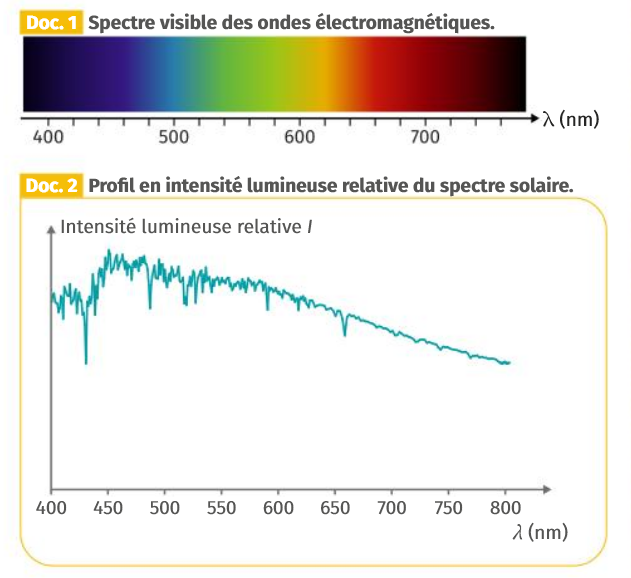
\includegraphics[width=\linewidth]{Ressources/2GT_C15_Ex_Fig1.png}
\end{center}
L'expression "Soleil jaune" est-elle justifiée d'après la longueur d'onde du maximum d'intensité lumineuse émise ?

\section{Les raies d'émission du lithium}
Le spectre d'émission du lithium est fourni ci-dessous.
\begin{center}
    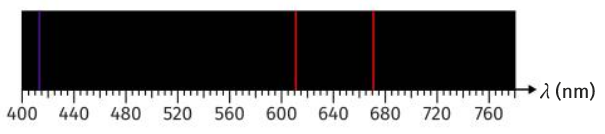
\includegraphics[width=\linewidth]{Ressources/2GT_C15_Ex_Fig2.png}
\end{center}
Montrer les trois longueurs d'onde des raies caractéristiques du lithium.

\section{Les réverbères au sodium}
Soumis à une excitation, les atomes de sodium émettrent deux raes caractéristiques de couleur jaune-orange, relativement proches l'une de l'autre en termes de longueur d'onde.
\begin{center}
    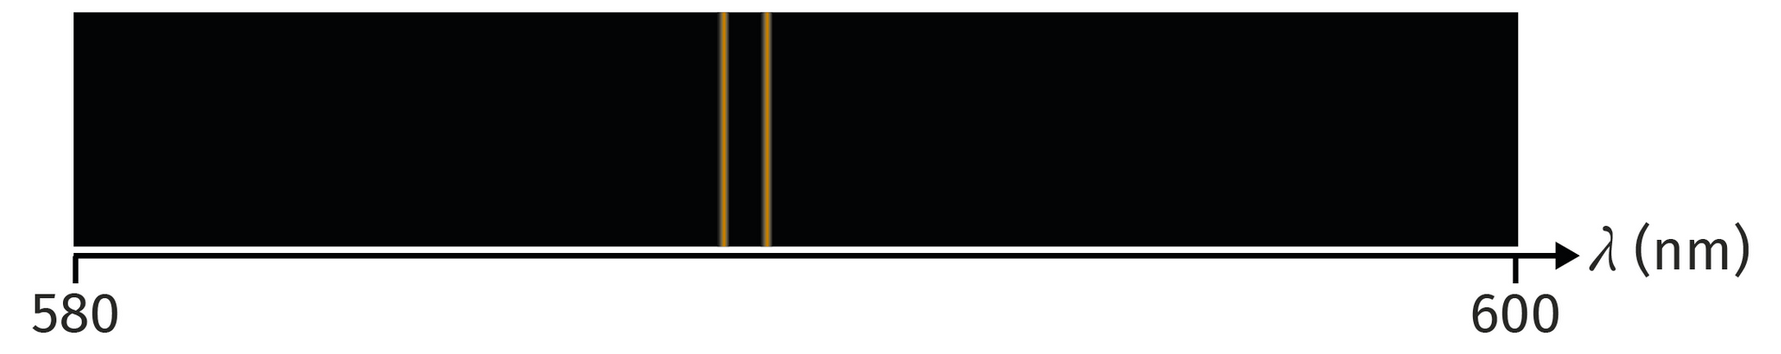
\includegraphics[width=\linewidth]{Ressources/2GT_C15_Ex_Fig3.png}
\end{center}
Déterminer avec le plus de précision possible les longueurs d'onde des deux raies caractéristiques et évaluer l'incertitude de cette mesure.

\section{La course autour de la Terre}
Fictivement, on imagine une course entre le son et la lumière autour de la Terre. Les deux ondes se positionnent à l'équateur et se lancent au même moment.\\
Déterminer le nombre de routs $N$ que parvient à faire la lumière avant que le son n'en finisse un seul.\\
\textbf{Données :}
\begin{itemize*}
    \item \textbf{Rayon de la Terre :} $R_T = \SI{6370}{km}$
    \item \textbf{Circonférence d'une sphère :} $C=2\pi R$
\end{itemize*}

\end{multicols}
\end{document}